\documentclass{article}

% Packages
\usepackage{hyperref}
\usepackage{color}
\usepackage{tocloft}
\usepackage{background}
\usepackage{graphicx}
\usepackage[a4paper, total={6in, 8in}]{geometry}
\usepackage{titlesec}
\usepackage[ddmmyyyy]{datetime}

% Settings
\definecolor{dark_primary_text}{cmyk}{0, 0, 0, 0.87}
\hypersetup{
  linktoc=all
}
\renewcommand{\cftsecleader}{\cftdotfill{\cftdotsep}}
\newcommand\DeactivateBG{\backgroundsetup{contents={}}}
\newcommand\ActivateBG{\backgroundsetup{
  scale = 1, angle = 0, opacity = 0.2,
  contents = {
    
\includegraphics[width = \paperwidth,height = \paperheight, keepaspectratio]{background.pdf}
  }
}}
\renewcommand{\dateseparator}{.}
\renewcommand{\contentsname}{Table of Contents}
\newcommand{\sectionbreak}{\clearpage}
\newcommand{\netgrif}{NETGRIF, s.r.o.}
\newcommand{\builder}{Netgrif Application Builder}
\newcommand{\version}{v0.3.0}
\newcommand{\engine}{Netgrif Application Engine}
\newcommand{\icon}[1]{ %! Suppress = FileNotFound
  \begingroup\normalfont
  \includegraphics[height=\fontcharht\font`\B]{#1}
  \endgroup

}

% Body
\color{dark_primary_text}
\begin{document}
  \begin{titlepage}
    \newgeometry{top=1in,bottom=0.5in,right=0.5in,left=0.5in}
    \ActivateBG
    \begin{center}
      \vspace*{9cm}
      \Huge
      \textbf{Netgrif Application Builder}\\
      \vspace{0.5cm}
      \LARGE
      \version \\
      \vspace*{\fill}
      \makebox[\linewidth]{\small \today}
    \end{center}
  \end{titlepage}
  \ActivateBG
  \newpage

  \section*{Changelog}\label{sec:changelog}
  \subsection*{0.4.0 - Silver Dysprosium (10.09.2020)}
  \subsubsection*{Bug Fixes}
    \begin{itemize}
      \item NAB-11 - Data variable editor text overflow
      \item NAB-95 - Arc data reference bug
      \item NAB-97 - Forms inconsistent in modeler
      \item NAB-107 - New added processes are not displayed in project overview
      \item NAB-117 - Data field ids generated as object Object
      \item NAB-118 - Form builder always displays calendar value selection
    \end{itemize}

  \subsubsection*{Improvements}
    \begin{itemize}
      \item NAB-62 - Form builder refactor
      \item NAB-124 - Select tool preselected by default on modeler screen
      \item NAB-125 - Add action button to transition context menu
    \end{itemize}

  \subsubsection*{Features}
    \begin{itemize}
      \item NAB-123 - File list data field
    \end{itemize}

\subsection*{0.3.0 - Aqua Neon (24.07.2020)}
  \subsubsection*{Bug Fixes}
    \begin{itemize}
      \item NAB-31 - Form builder - inconsistent number of cols
      \item NAB-28 - Dashboard tiles refresh
      \item NAB-25 - Actions has the same id
      \item NAB-24 - Transition actions have trigger PRE/POST
      \item NAB-17 - Custom field inconsistencies
      \item NAB-16 - Builder does not load on Firefox
      \item NAB-14 - XML special chars are not escaped
    \end{itemize}

  \subsubsection*{Improvements}
    \begin{itemize}
      \item NAB-100 - Form builder default values
      \item NAB-96 - Jenkins Pipeline
      \item NAB-51 - Custom data field export
    \end{itemize}

  \subsubsection*{Features}
    \begin{itemize}
      \item NAB-93 - I18n view
      \item NAB-91 - Modeler Tour
      \item NAB-77 - Automation policies
      \item Task icon is displayed in modeler in the middle of the transition rectangle
    \end{itemize}

  \subsubsection*{Tasks}
    \begin{itemize}
      \item NAB-8 - Datetime field refactor
    \end{itemize}

\subsection*{0.2.0 - Navy Hafnium}
  \subsubsection*{Features}
    \begin{itemize}
      \item resizable action editor
      \item tables can be sorted by clicking on its headers
      \item side editors can be resized
      \item data fields options can be edited in the Data variable editor
    \end{itemize}


  \DeactivateBG
  \restoregeometry
  \tableofcontents
  \newpage

  \section{Introduction}\label{sec:introduction}
  \builder~is a web application focused on developing process-driven applications using the \engine.
\engine~provides a platform that allows you to model and automate business processes as a sequence of tasks performed
in accordance with defined rules, integrate tasks from existing applications into processes, while digitizing "paper"
tasks with the need to program only to the extent necessary.

Workflow processes are implemented within Netgrif AE using the so-called workflow nets that consist of state variables,
tasks and their interconnections.
Workflow nets determine where individual tasks can be performed.

Reports of enabled tasks and processed tasks can be displayed in different forms according to customer requirements,
for example in the form of graphs or tables.
After choosing a Dashboard task type, the user will be able to access a list of tasks of the type in the Task Manager screen.

Individual tasks in Task Manager can be assigned to users based on predefined roles (delegate).
Upon assignment, the status of the task changes from the enabled state to the assigned state.
The assigned task can be canceled or moved to another user with the same rights (reassign).

The application allows using customized filtering to create personalized task lists.
Personalized task lists can be created by the user himself or created by a supervisor.
In user management, it is possible to assign specific users to roles and groups within the customer's organizational structure.


  \section{Views}\label{sec:views}
  The \builder~consists of multiple views:

\begin{itemize}
  \item[\icon{images/icons/projects.png}] projects overview
  \item[\icon{images/icons/project.png}] project detail
  \item[\icon{images/icons/modeler.png}] modeler
  \item[\icon{images/icons/form.png}] form builder
  \item[\icon{images/icons/dashboard.png}] dashboard builder
\end{itemize}
Each view is accessible from the left navigation rail by clicking on the view icon.


  \section{Projects Overview}\label{sec:projects-overview}
  Projects overview displays all user's projects and allows users to create a new project or import an existing project (Figure~\ref{fig:projects_overview}).
The project list shows the title and description of each project in a separate line.
After clicking on a project its line expands and processes are displayed in a form of chips.
Each chip shows the process icon and title.
At the bottom of the expanded line there are buttons for managing the process.
Delete button will permanently remove the project.
Open button will navigate the user to \hyperref[sec:project-detail]{Project Detail} view.

\begin{figure}[h!]
  \centering
  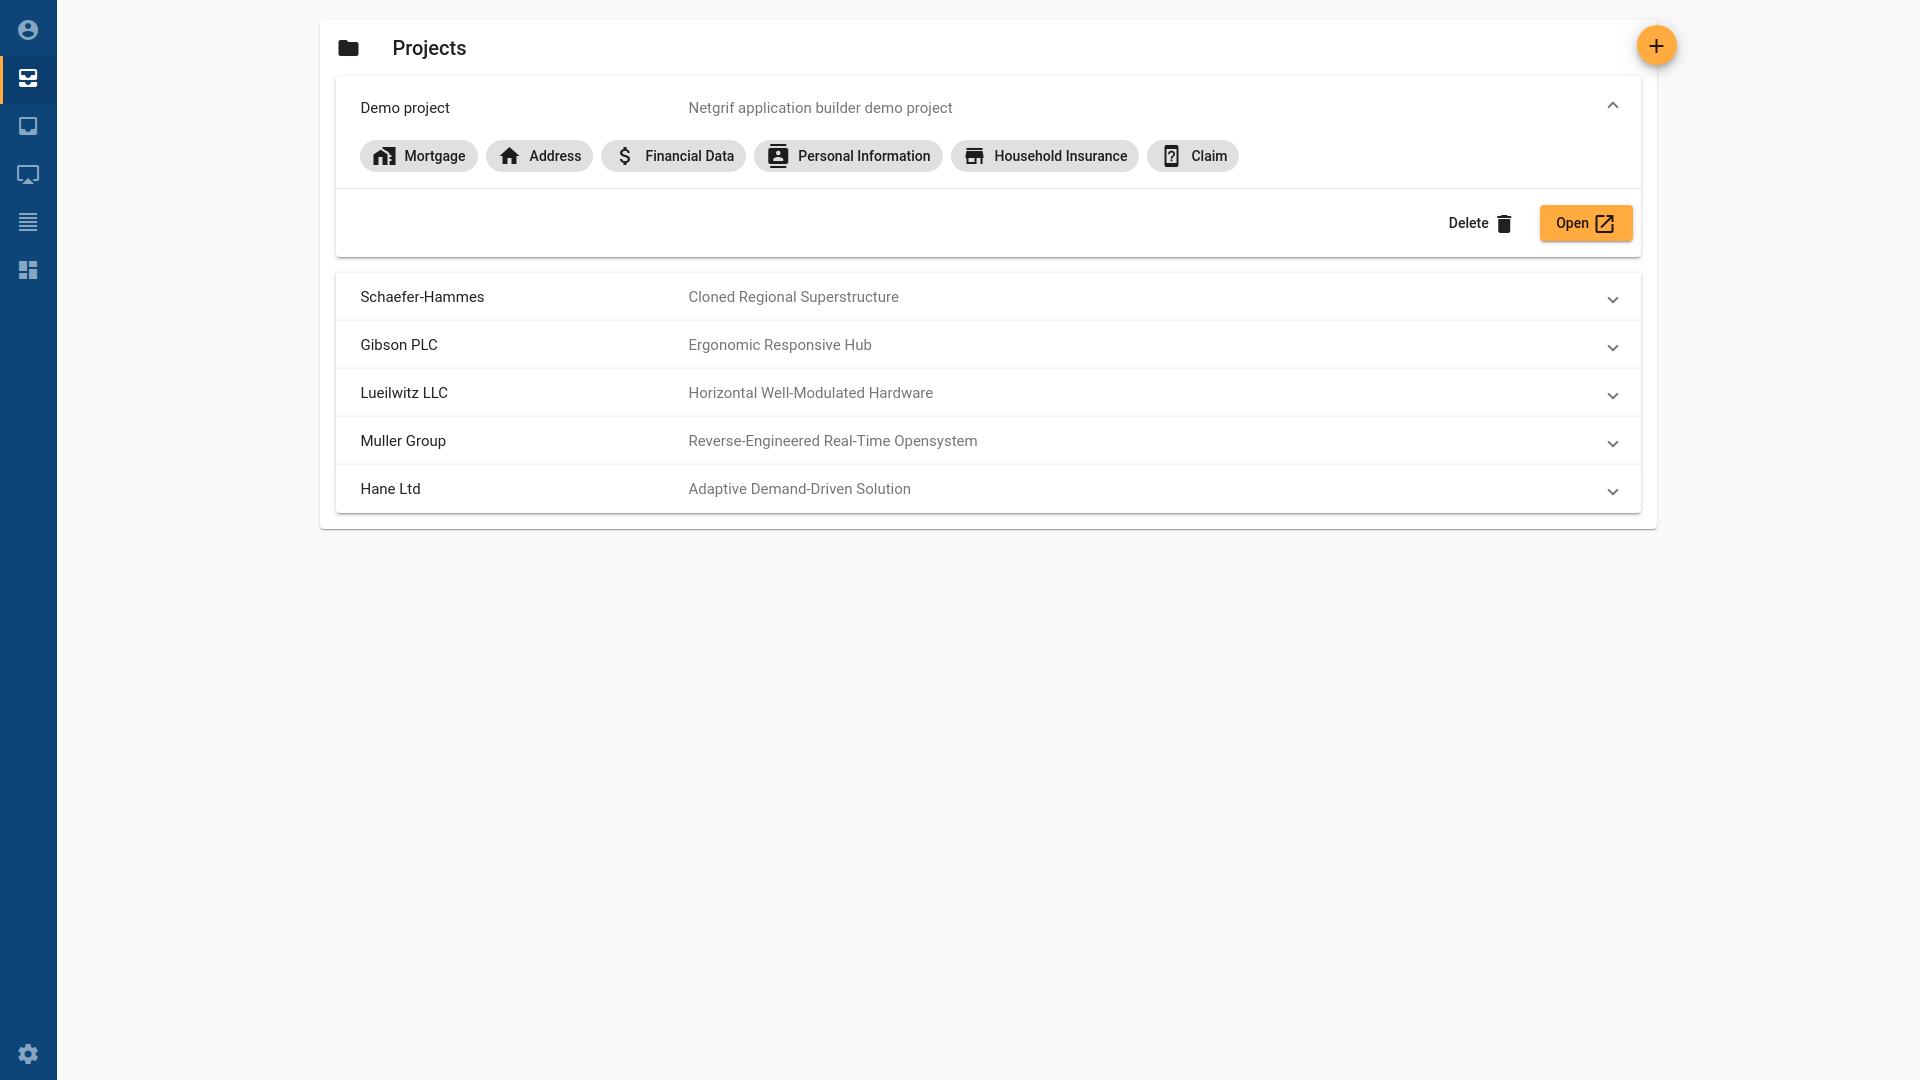
\includegraphics[width=0.9\textwidth]{images/projects_view.png}
  \caption{Projects overview}
  \label{fig:projects_overview}
\end{figure}

Clicking on the fast action button on the right side will show two options for creating a new project.
The first option is to create a new empty project.
Importing an existing project is the other option, which will open a file dialog where you can select an existing project on your device.

Projects are currently not saved to any server and leaving the \builder~will result in the loss of all projects.


  \section{Project Detail}\label{sec:project-detail}
  
Project detail consists of two main sections divided into separate cards: project information and a list of processes (Figure~\ref{fig:project_detail}).

\begin{figure}[h!]
  \centering
  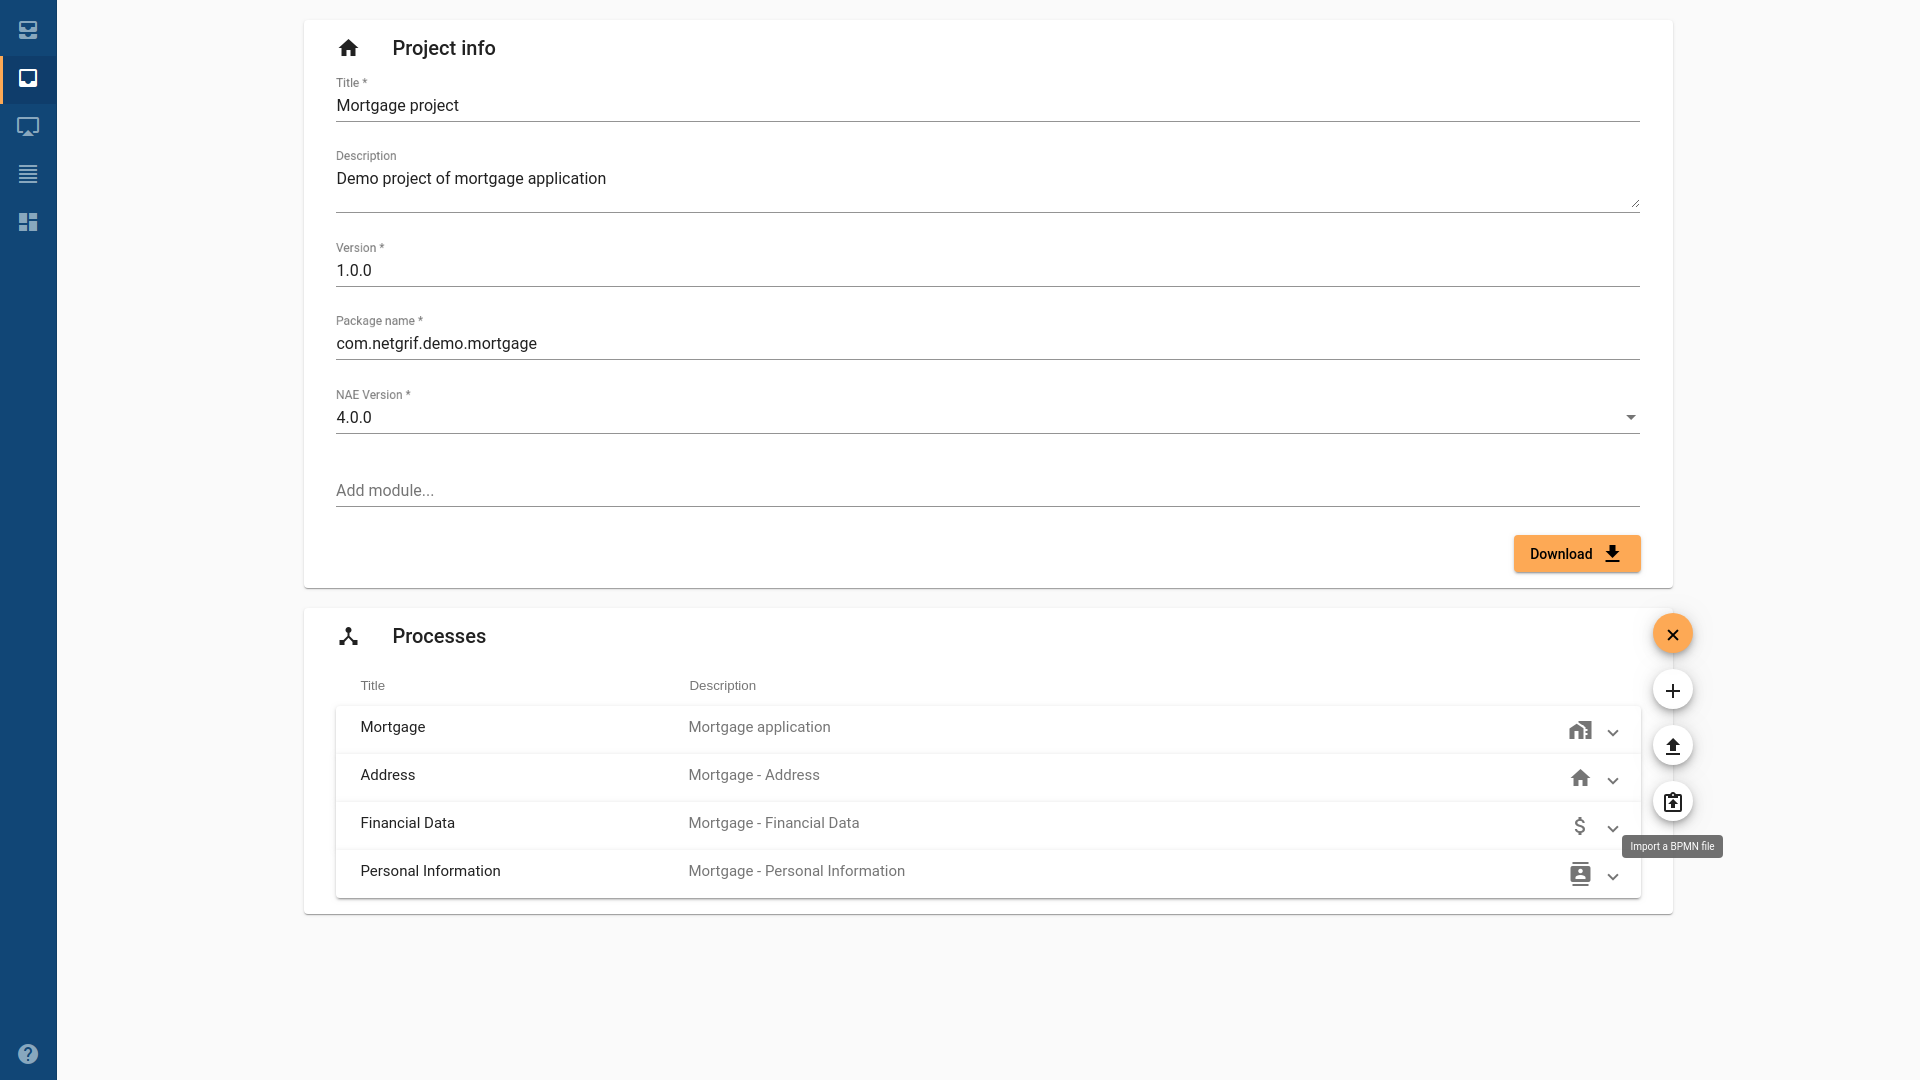
\includegraphics[width=0.9\textwidth]{images/project_view.png}
  \caption{Project detail}
  \label{fig:project_detail}
\end{figure}

\subsection{Project Info}\label{subsec:project-info}

Project info card shows all project metadata in an editable form:
\begin{itemize}
  \item title,
  \item description,
  \item version,
  \item package name - the name of the base Java package,
  \item NAE version - version of \engine~that will be used to run this project,
  \item modules.
\end{itemize}
Changes to any field are automatically saved.

At the bottom of the card, there is a \texttt{Download} button that will compress the project configuration file and all processes into a single zip file.
Projects are currently not saved to any server and leaving the \builder~will result in the loss of all projects.

\subsection{Processes}\label{subsec:processes}

This card shows a list of all processes in the current project.
Processes are sorted in the order as they were created.
To change the sorting simply click on the \texttt{Title} of \texttt{Description} header.
After each click the sorting cycles through different orders as follows: ascending order, descending order and no order.

Each process is initially displayed as a single list item showing its title, description and icon.
After clicking on the process the item expands and additional data are shown in an editable form:
\begin{itemize}
  \item title,
  \item case title - default title of a new case,
  \item description,
  \item version,
  \item initials,
  \item icon - any Material Design icon can be used, a list of all icons is available at \url{https://material.io/resources/icons/},
  \item identifier - unique string identifying the process.
\end{itemize}
Changes to any field are automatically saved.
At the bottom of the process detail there are two buttons \texttt{Delete} and \texttt{Open}.
Clicking on the Delete button deletes the process.
Clicking on the Open button will redirect you to the \hyperref[sec:modeler]{Modeler view} where the process is displayed.

A new process can be added to the project by clicking the fast action button on the right border of the card and selecting one of the following options:
\begin{itemize}
  \item new process - creates an empty process model,
  \item import an existing process - opens a file dialog where you can choose an XML file of a Petriflow model,
  \item import a BPMN file - opens a file dialog where you can choose a BPMN file which will be transformed and imported into the project.
\end{itemize}
After that a new item is added to the list of processes.


  \section{Modeler}\label{sec:modeler}
  The Modeler allows the user to simply create and edit all processes of the project using the following components:
\begin{itemize}
  \item process editor,
  \item process simulator,
  \item data variable editor,
  \item role editor,
  \item action editor.
\end{itemize}
These components are accessible from the Modeler toolbar by clicking on its icon.
Above the toolbar, there are tabs for each process of the project and a tab with a plus icon which can be used to create a new process.

\subsection{Process editor}\label{subsec:process-editor}

In the process editor component the selected process is displayed.
The upper toolbar contains tools for working with the whole process (import, export, clear, etc.), editing places and transitions (add new, change marking, change label, etc.), editing arcs (create new regular, reset, inhibitor, or read arc, change multiplicity, etc.), and working with the layout (auto align elements, move element, etc.).
Task icons are displayed in the middle of the transition rectangle.

\begin{figure}[h!]
  \centering
  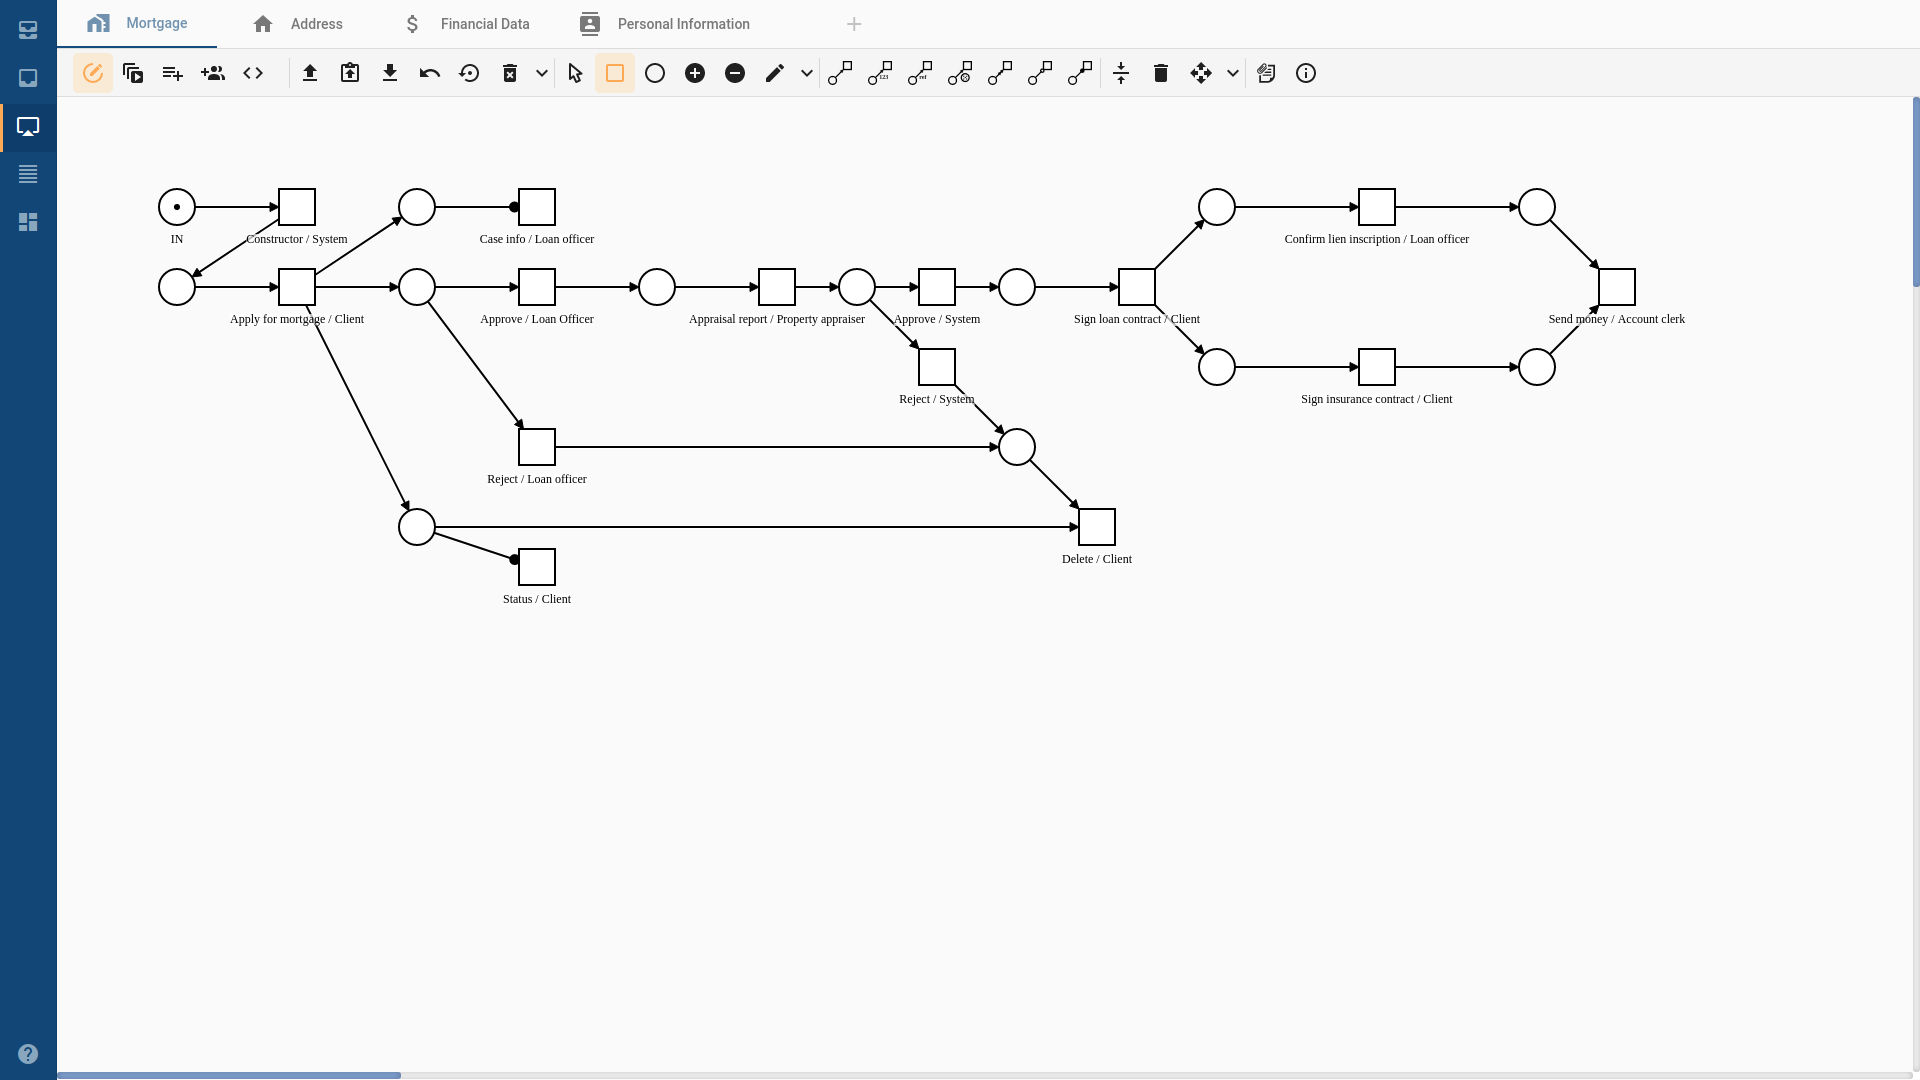
\includegraphics[width=0.9\textwidth]{images/modeler_process_editor.png}
  \caption{Modeler - process editor}
  \label{fig:modeler_process_editor}
\end{figure}

\subsection{Process simulator}\label{subsec:process-simulator}

This view allows users to simulate the execution of a given process (Figure~\ref{fig:modeler_process_simulator}).
There are two modes for different types of simulation - transition mode and task mode.
In both modes enabled tasks are shown with a green border and background.
Inactive tasks are shown with a red border.

In the transition mode clicking on an enabled task will execute it immediately.
Tokens from input places are consumed and new tokens are produced in the output places as defined by the Petri net.

Task mode simulates real execution of the task as it is implemented in the \engine.
Clicking on an enabled task simulates assigning of the given task.
Tokens from input places are consumed and two arrows displayed in the center of the task.
The red arrow cancels the execution, the green arrow will finish the execution and produce new tokens in the output places as defined by the Petri net.

\begin{figure}[h!]
  \centering
  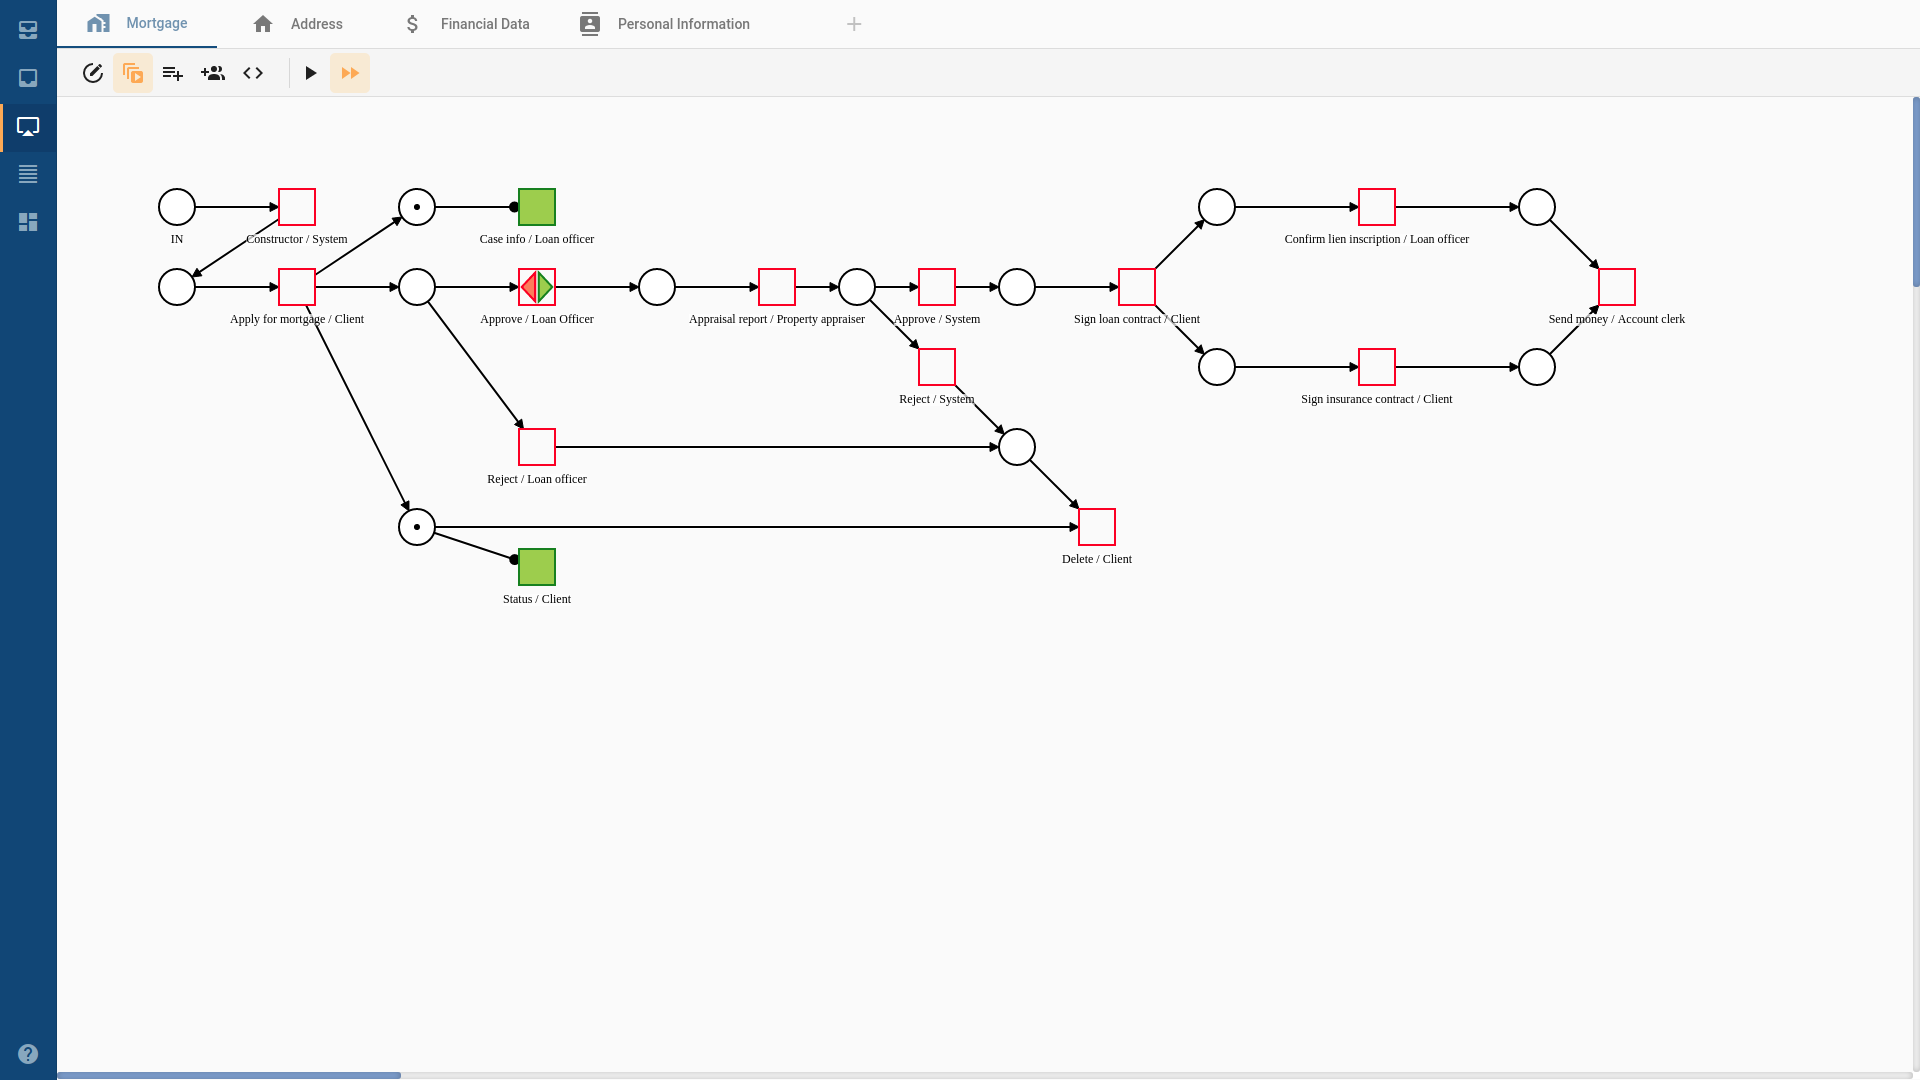
\includegraphics[width=0.9\textwidth]{images/modeler_process_simulator.png}
  \caption{Modeler - process simulator}
  \label{fig:modeler_process_simulator}
\end{figure}

\subsection{Data variable editor}\label{subsec:data-variable-editor}

Data variables are displayed as a master-detail interface (Figure~\ref{fig:modeler_data_editor}).
The master list contains all data variables and allows users to select it by clicking.
The selected data variable is displayed in the detail as an editable form.
All changes are automatically saved.
A data variable can be deleted by clicking the \texttt{Delete data field} button which is displayed while the cursor is above the field's item in the list.

\begin{figure}[h!]
  \centering
  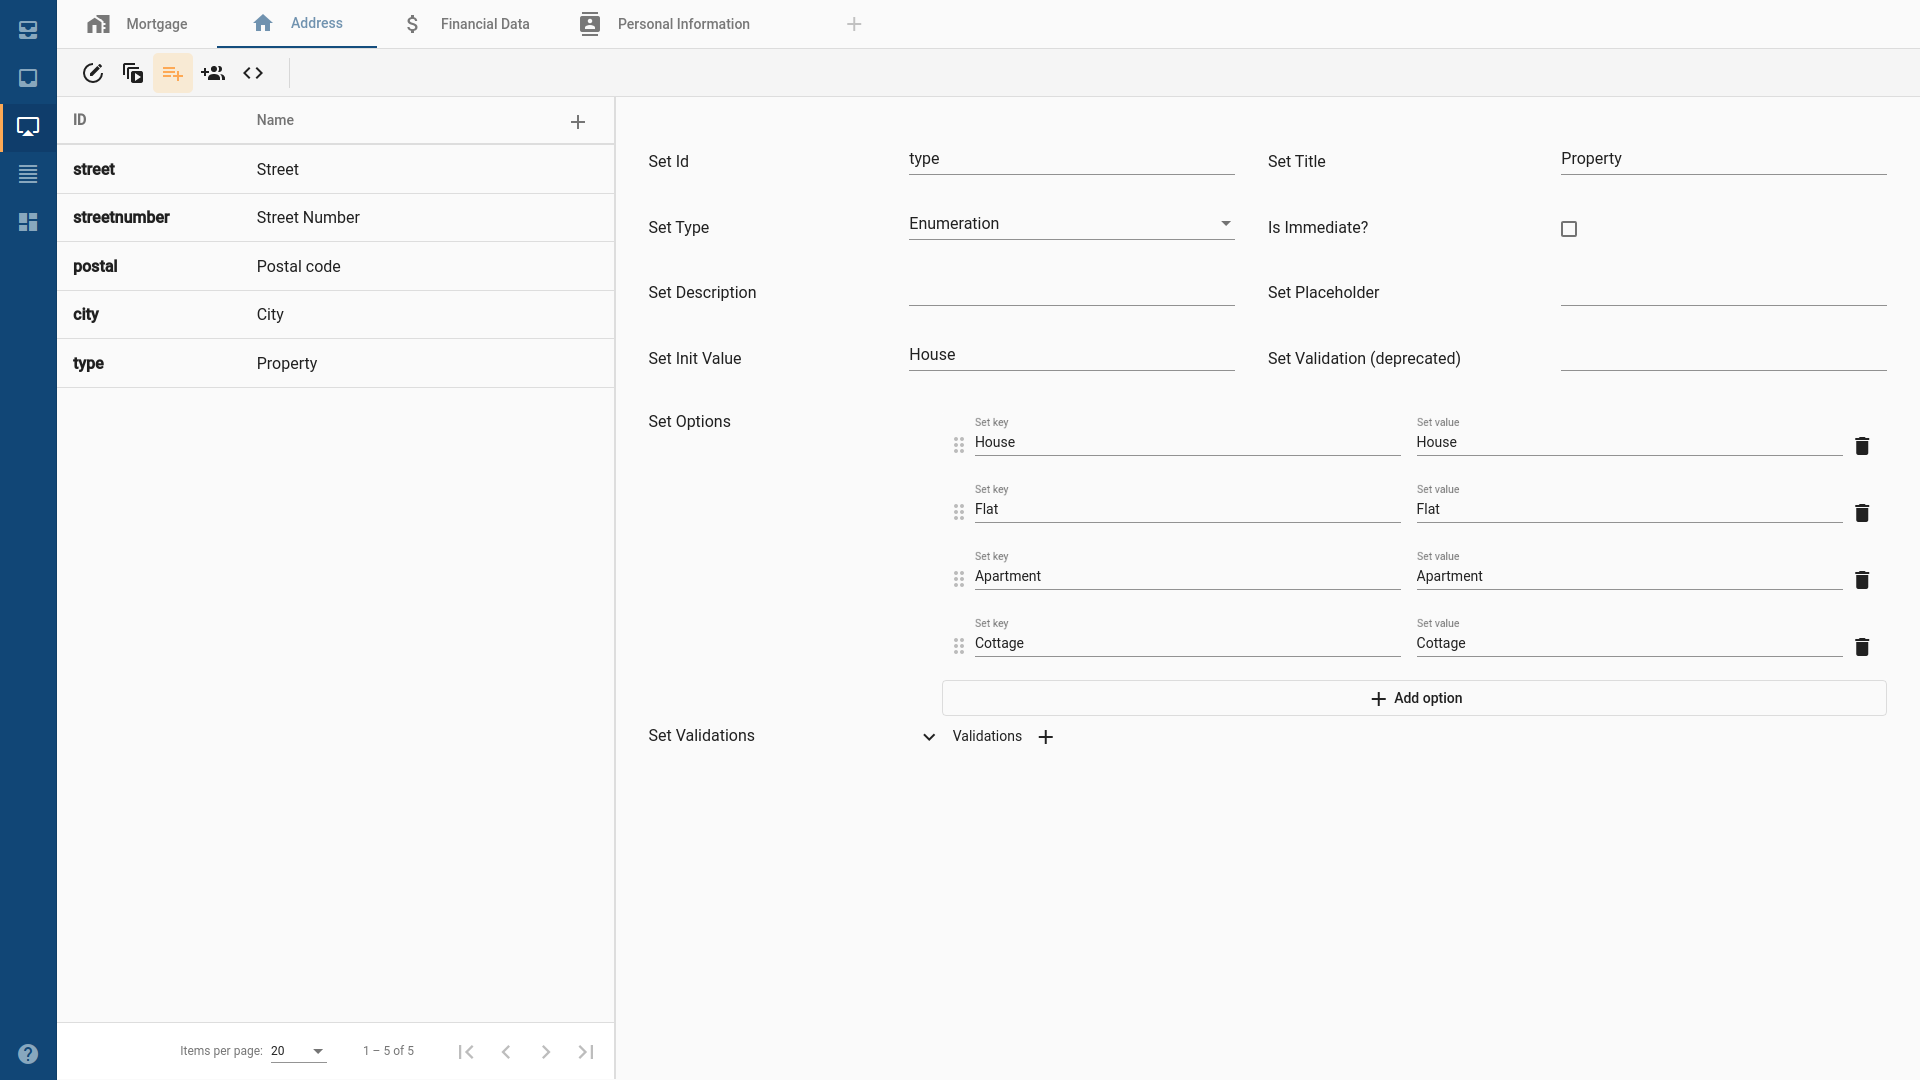
\includegraphics[width=0.9\textwidth]{images/modeler_data_editor.png}
  \caption{Modeler - data variable editor}
  \label{fig:modeler_data_editor}
\end{figure}

\subsection{Role editor}\label{subsec:role-editor}

The Role editor displays all roles of the given process in a pageable list (Figure~\ref{fig:modeler_role_editor}).
Each item shows only id and title, which can be edited after clicking on the list and expanding it into an editable form.
Changes to any field are automatically saved.
Clicking the \texttt{Delete} button at the bottom will permanently remove the role.

\begin{figure}[h!]
  \centering
  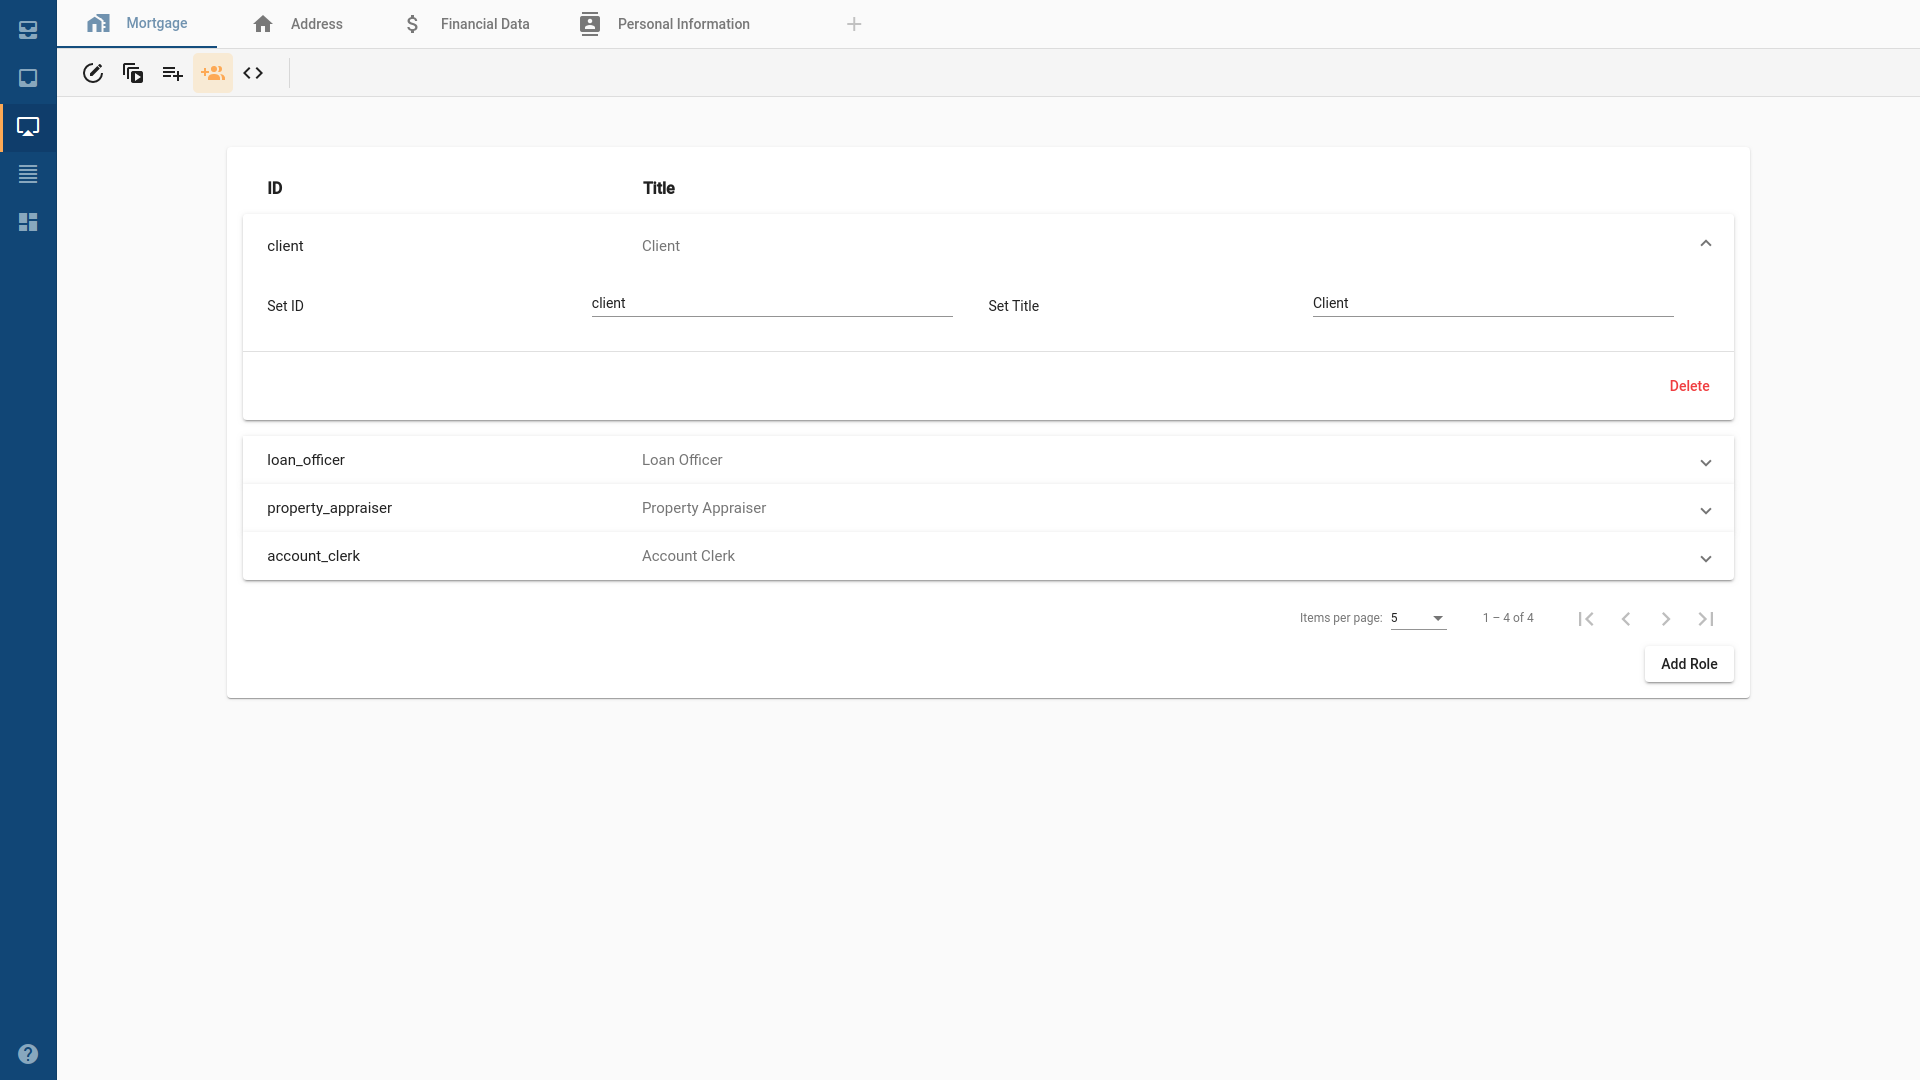
\includegraphics[width=0.9\textwidth]{images/modeler_role_editor.png}
  \caption{Modeler - role editor}
  \label{fig:modeler_role_editor}
\end{figure}

\subsection{Action editor}\label{subsec:action-editor}

The action editor allows users to view, add, and edit actions of the given process as a master-detail interface (Figure~\ref{fig:modeler_action_editor}).
In the editor's toolbar, the user can choose between actions bound to data variables or tasks.

The first option will show a list of all data variables in the master list.
Selecting a data field will show a list of actions categorized by its trigger in the detail.
A new action can be added by clicking on the plus button next to the trigger category.
After expanding the action by clicking on it a code editor is displayed where the user can write the action body.
The code editor shows 10 lines of code by default, but can be resized by dragging the bottom border of the whole action card.

The other option will show a list of all tasks and allows to edit actions bound to events or data fields of the given task.

\begin{figure}[h!]
  \centering
  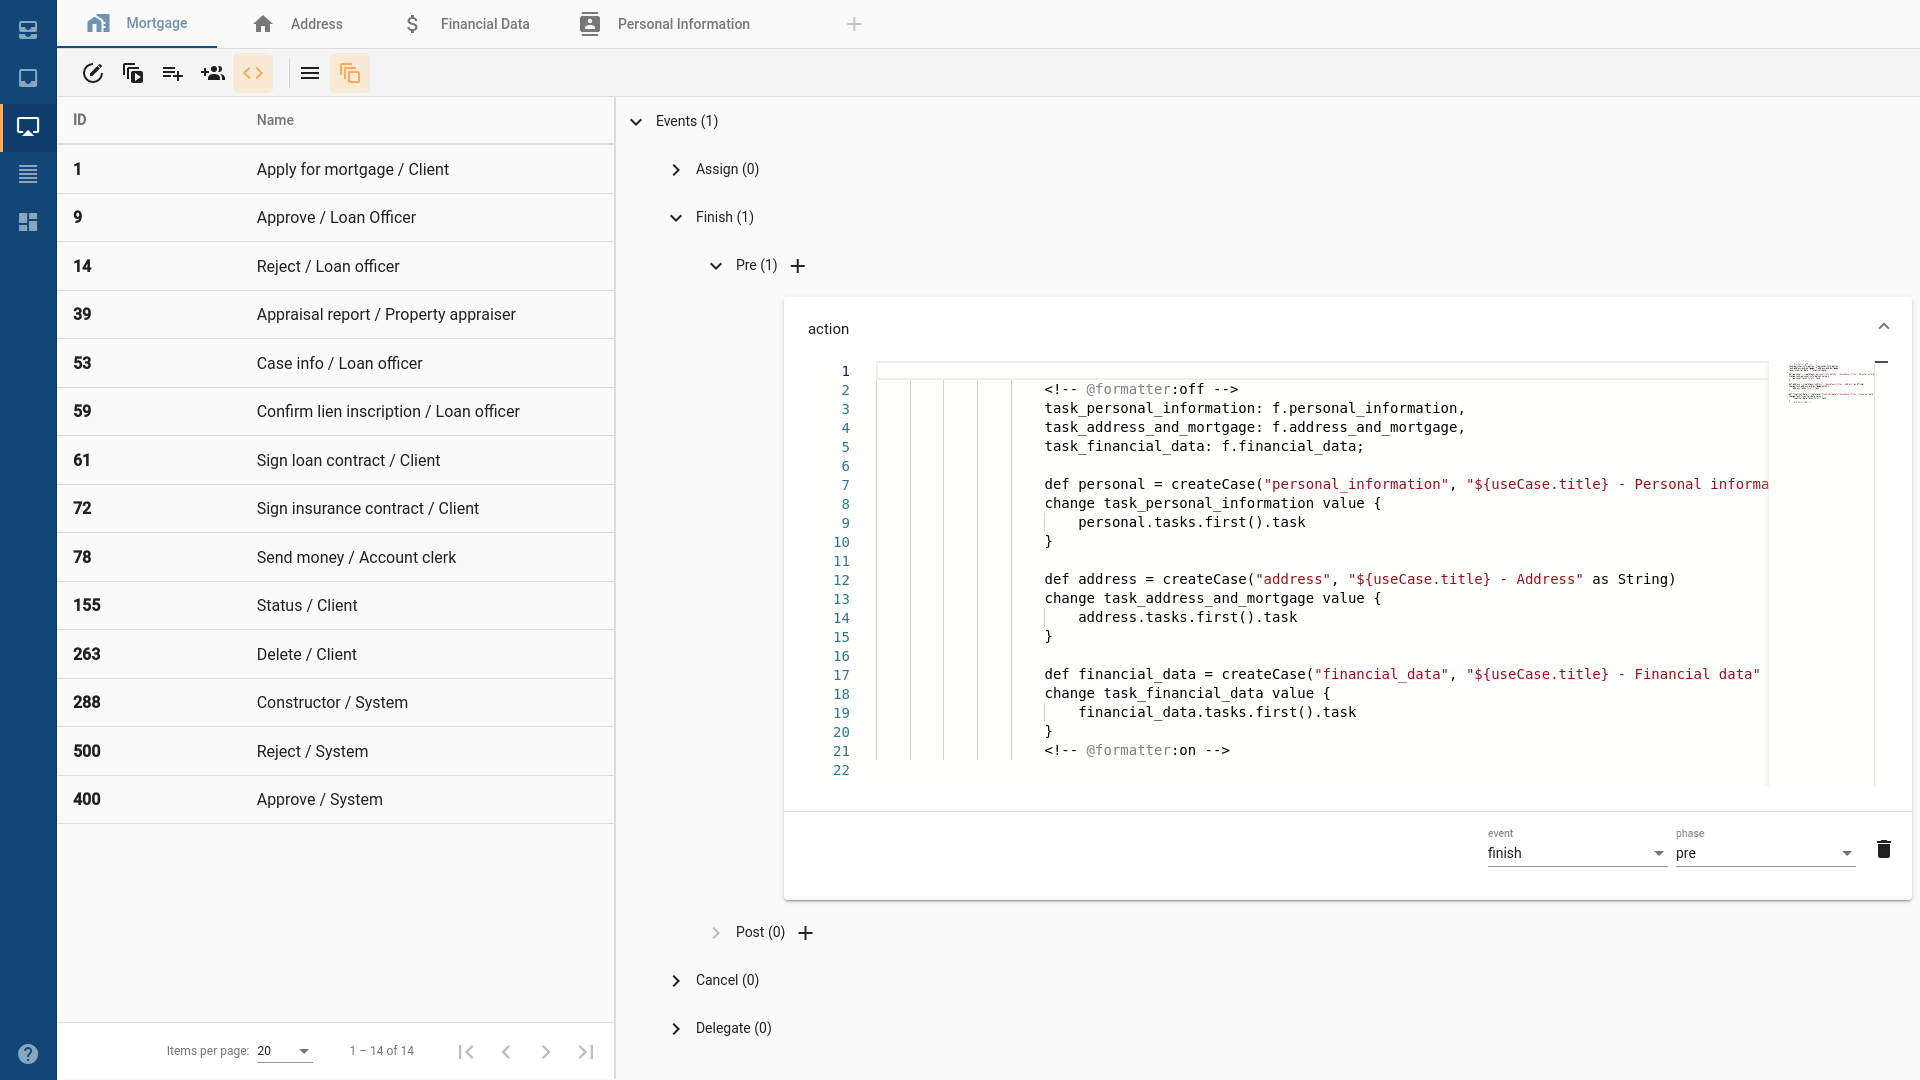
\includegraphics[width=0.9\textwidth]{images/modeler_action_editor.png}
  \caption{Modeler - action editor}
  \label{fig:modeler_action_editor}
\end{figure}


  \section{Form Builder}\label{sec:form-builder}
  The Form Builder allows users to assign a form to a task and customize its data fields (Figure~\ref{fig:form_builder}).

The forms data fields are displayed in the centre of the screen in a grid layout.
The number of columns of the grid layout can be modified in the right side panel.
The default value is 4 columns.
The minimal number of columns is 2 and maximal is 6.

Data field can be placed in the layout by dragging it from the left side panel where all types of data fields are available.
At the bottom of the list are all fields that exist in the given process.
Existing fields that are already used in the current form are disabled for dragging.

Further customization of data field style is possible by creating a custom field by clicking the fast action button on the right border of the left side panel.
A dialog is then opened where the user has to select the fields type and title and insert the custom HTML and CSS\@.
After clicking the Save button the new field is added to the list in the left side panel and ready to use.

Data field can be selected by clicking on it.
Settings of the selected data field are shown in the right side panel where you can edit the following properties:
\begin{itemize}
  \item behavior,
  \item netgrif template,
  \item style,
  \item label,
  \item placeholder,
  \item description,
  \item value,
  \item options (only available for enumeration and multichoice fields).
\end{itemize}
Any change is automatically saved.

\begin{figure}[h!]
  \centering
  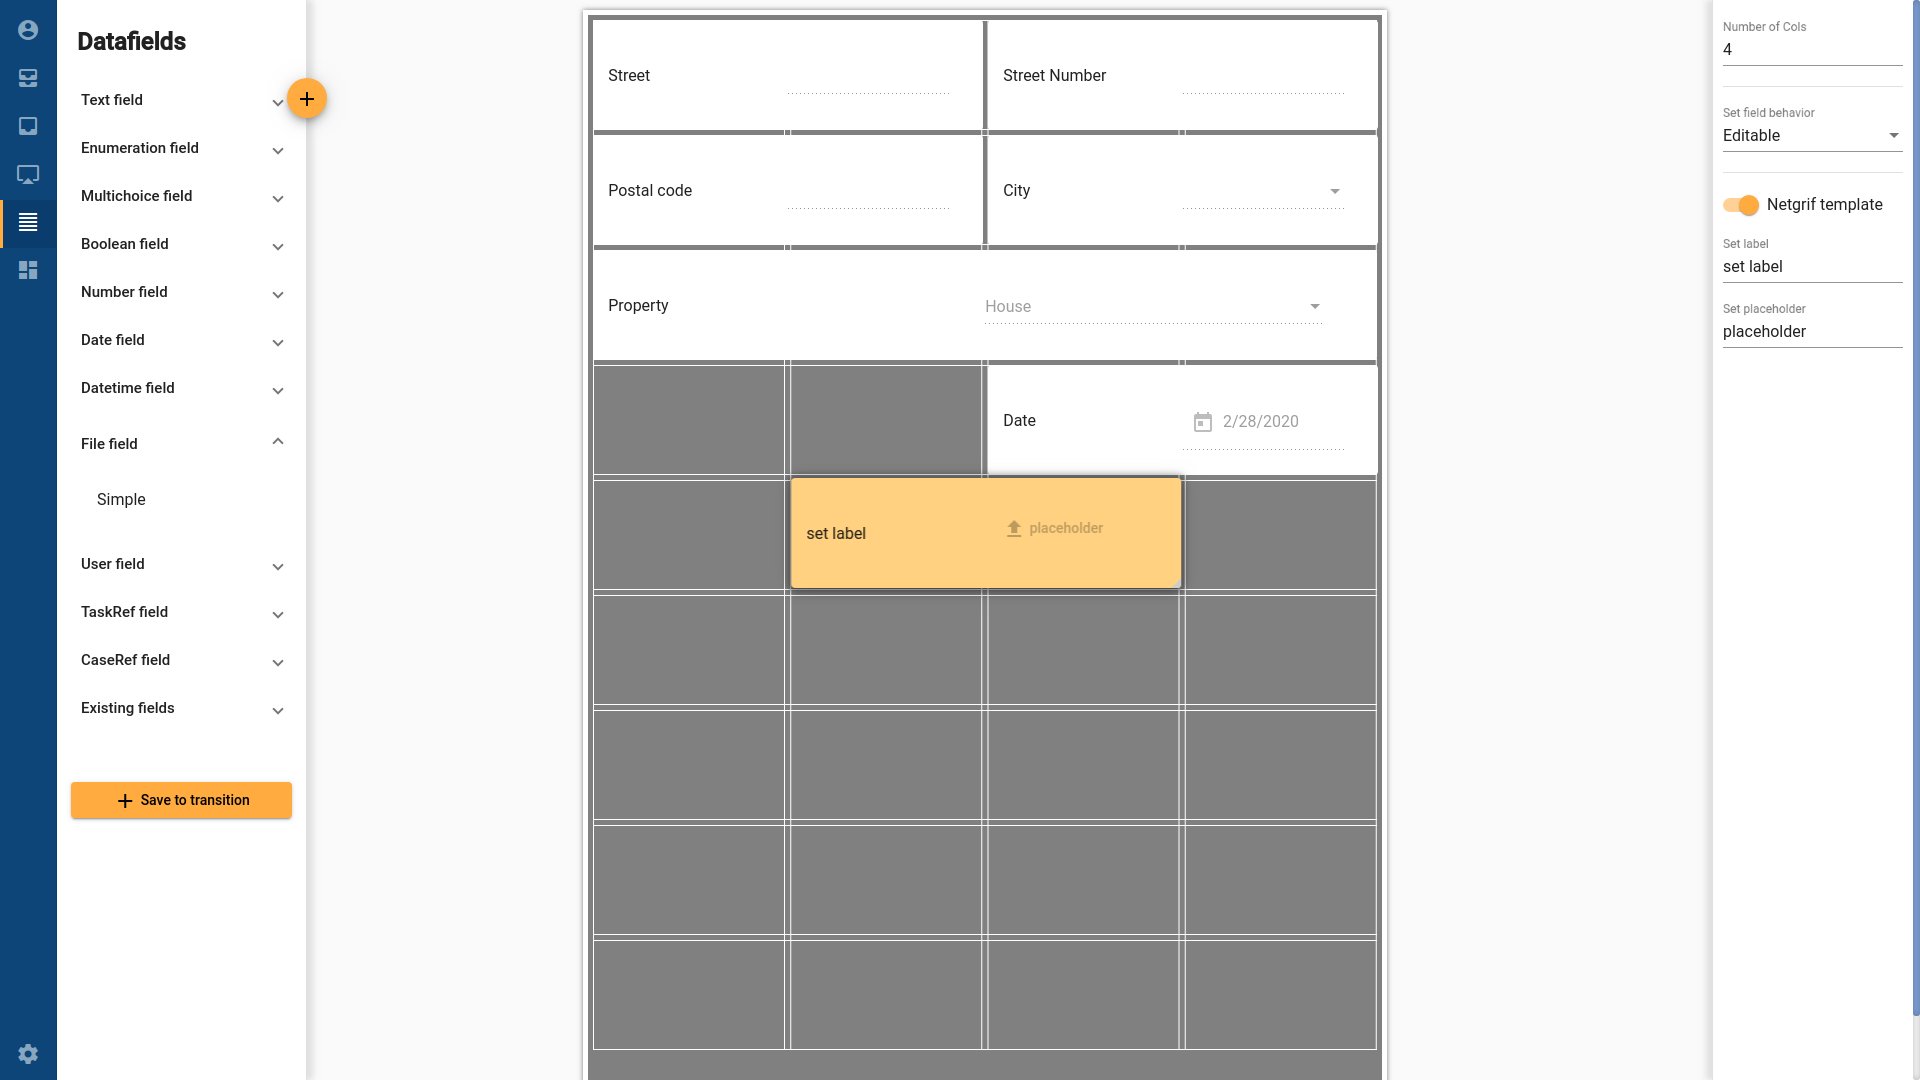
\includegraphics[width=0.9\textwidth]{images/form_view.png}
  \caption{Form builder}
  \label{fig:form_builder}
\end{figure}


  \section{Dashboard}\label{sec:dashboard}
  Dashboard view displays a grid that is used to create and arrange visualisations (Figure~\ref{fig:dashboard}).
By clicking on an empty cell you can create a new empty visualisation with default settings.
By clicking and dragging on empty cells you can define the size of the new visualisation.
Existing visualisations can be resized by simply dragging their borders in the desired direction.
By clicking and dragging on an existing visualisation you can change its position in the grid.
To delete a visualisation click on the button in the upper right corner of the visualisation.

Editing mode is activated by clicking on an existing visualisation.
Settings of the selected visualisation are shown on the right side panel.
In this panel you can change:
\begin{itemize}
  \item title,
  \item type,
  \item URL,
  \item request.
\end{itemize}
All changes are automatically saved.
Supported visualisation types are:
\begin{itemize}
  \item area chart,
  \item bar chart,
  \item line chart,
  \item pie chart,
  \item metric.
\end{itemize}

\begin{figure}
  \centering
  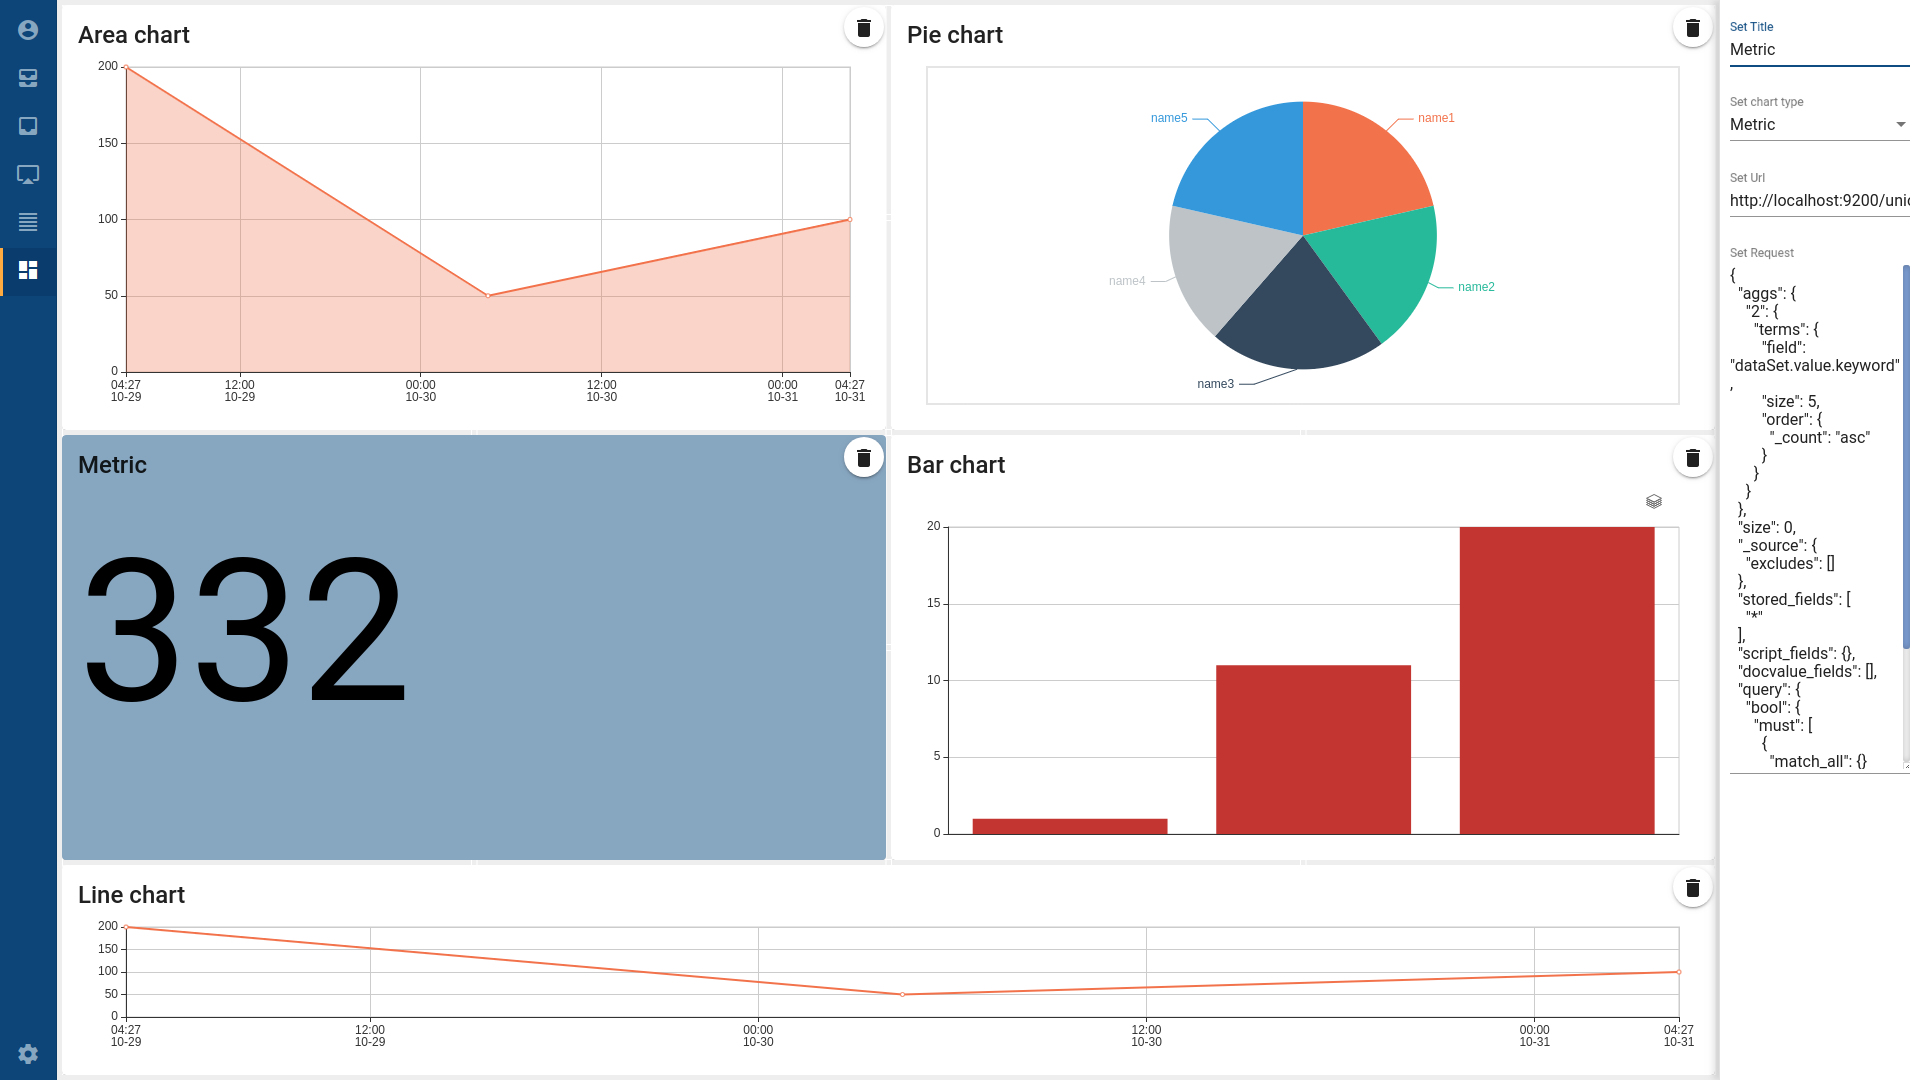
\includegraphics[width=0.9\textwidth]{images/dashboard_view.png}
  \caption{Dashboard view}
  \label{fig:dashboard}
\end{figure}

\subsection{Elasticsearch and Kibana}\label{subsec:elasticsearch-and-kibana}

Data for visualisation are loaded from an Elasticsearch instance running on the specified URL\@.
Elasticsearch query has to be specified in the request field.
You can use Kibana for creating the request.
Create a new visualisation in Kibana following the official tutorial on \url{https://www.elastic.co/guide/en/kibana/current/tutorial-visualizing.html}.
On the top toolbar click on the Inspect button.
This will open a side panel with more details about the visualisation including raw data, statistics, request, and response.
From the \texttt{View} dropdown menu on the right select \texttt{Request} and switch to the \texttt{Request} tab.
Finally, copy the request body into the request field of a dashboard visualisation in the \builder.


\end{document}
